\documentclass{article}
% 夾帶 fixture 共用的樣式：只用 TikZ 內建與常見函式庫，字為 ASCII，不需要 CJK 字型。
\usepackage{tikz}
\usetikzlibrary{arrows.meta,positioning,fit,backgrounds,shapes.geometric,calc}
\tikzset{
  box/.style={rectangle, rounded corners=3pt, draw, fill=blue!8, minimum height=8mm, minimum width=22mm, align=center},
  decision/.style={diamond, aspect=2.4, draw, fill=gray!8, align=center, inner sep=2pt},
  flow/.style={-{Stealth[length=2.5mm]}, thick},
  lab/.style={font=\scriptsize, fill=white, inner sep=2pt},
  annot/.style={rectangle, draw, dashed, fill=white, font=\footnotesize, align=center},
  leader/.style={densely dotted, shorten >=2pt, shorten <=2pt},
  region/.style={draw, dashed, rounded corners=4pt, fill=gray!6, inner sep=8pt},
}

\begin{document}

% 每張圖只犯一條規則；test.sh 比對每張圖回報的規則集合與 expect 是否相同。

% expect: node-overlap
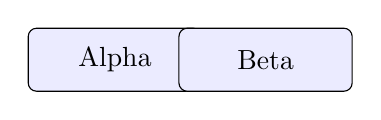
\begin{tikzpicture}
  \node[box] (a) {Alpha};
  \node[box, right=-3mm of a] (b) {Beta};
\end{tikzpicture}

% 間距不足：兩框幾乎貼在一起
% expect: node-overlap
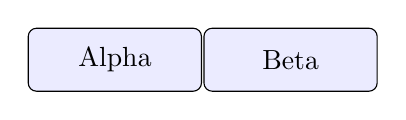
\begin{tikzpicture}
  \node[box] (a) {Alpha};
  \node[box, right=0.5pt of a] (b) {Beta};
\end{tikzpicture}

% 外框切過不屬於它的節點
% expect: node-overlap
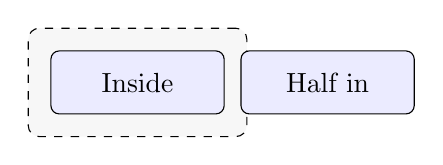
\begin{tikzpicture}
  \node[box] (a) {Inside};
  \node[box, right=2mm of a] (c) {Half in};
  \begin{scope}[on background layer]
    \node[region, fit=(a)] {};
  \end{scope}
\end{tikzpicture}

% expect: edge-through-node
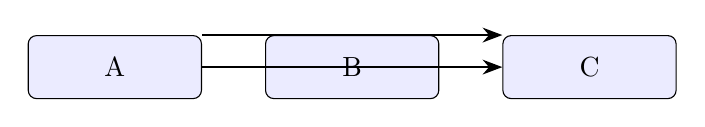
\begin{tikzpicture}[node distance=8mm]
  \node[box] (a) {A};
  \node[box, right=of a] (b) {B};
  \node[box, right=of b] (c) {C};
  \draw[flow] (a.north east) to[bend left=0] (c.north west);
  \draw[flow] (a) -- (c);
\end{tikzpicture}

% 白底標籤比兩節點的間隔寬
% expect: label-on-node
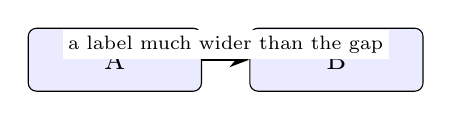
\begin{tikzpicture}
  \node[box] (a) {A};
  \node[box, right=6mm of a] (b) {B};
  \draw[flow] (a) -- node[lab, above] {a label much wider than the gap} (b);
\end{tikzpicture}

% 沒有白底的裸字標籤一樣算
% expect: label-on-node
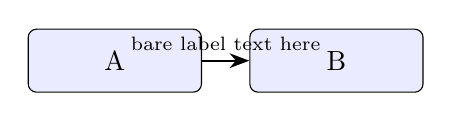
\begin{tikzpicture}
  \node[box] (a) {A};
  \node[box, right=6mm of a] (b) {B};
  \draw[flow] (a) -- node[font=\scriptsize, above] {bare label text here} (b);
\end{tikzpicture}

% expect: label-on-label
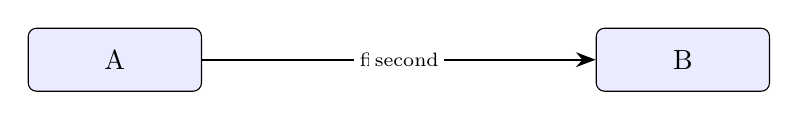
\begin{tikzpicture}
  \node[box] (a) {A};
  \node[box, right=50mm of a] (b) {B};
  \draw[flow] (a) -- node[lab, pos=0.45] {first} node[lab, pos=0.52] {second} (b);
\end{tikzpicture}

% expect: label-on-arrow
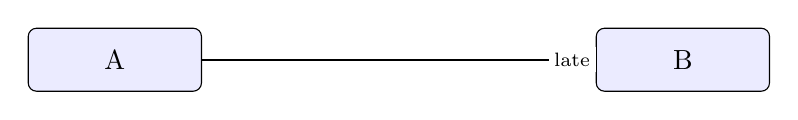
\begin{tikzpicture}
  \node[box] (a) {A};
  \node[box, right=50mm of a] (b) {B};
  \draw[flow] (a) -- node[lab, pos=0.94] {late} (b);
\end{tikzpicture}

% 固定 text width 放不下的長字
% expect: text-overflow
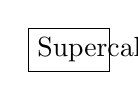
\begin{tikzpicture}
  \node[draw, text width=8mm] {Supercalifragilistic};
\end{tikzpicture}

% 菱形：字在外框（bounding box）內，但角落伸出斜邊
% expect: text-overflow
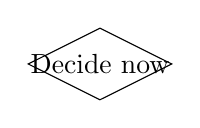
\begin{tikzpicture}
  \node[diamond, draw, aspect=2, inner sep=-2pt] {Decide now};
\end{tikzpicture}

% expect: edge-overlap
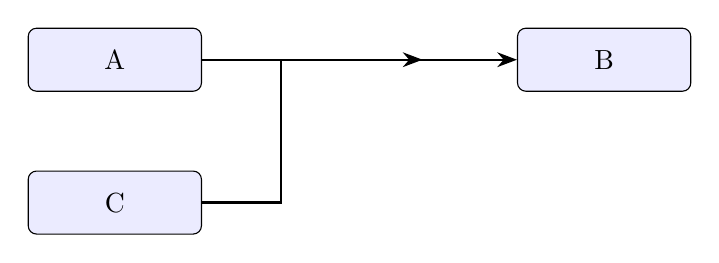
\begin{tikzpicture}
  \node[box] (a) {A};
  \node[box, right=40mm of a] (b) {B};
  \node[box, below=10mm of a] (c) {C};
  \draw[flow] (a) -- (b);
  \draw[flow] (c.east) -- ++(10mm,0) |- ([xshift=-12mm]b.west);
\end{tikzpicture}

% 只有給 --max-width 10cm 時才檢查
% expect: figure-width
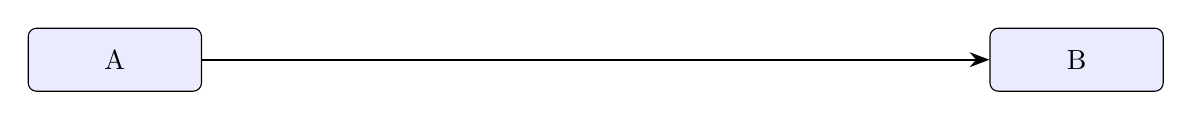
\begin{tikzpicture}
  \node[box] (a) {A};
  \node[box, right=100mm of a] (b) {B};
  \draw[flow] (a) -- (b);
\end{tikzpicture}

% 圖本身編不過：只擋這一張，其他圖照常量測
% expect: compile
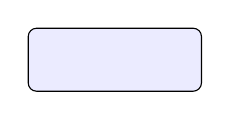
\begin{tikzpicture}
  \node[box] {\undefinedcommand};
\end{tikzpicture}

% 刻意的壓疊以註記放行，只對這張圖、只對列出的規則
% tikz-guard: allow node-overlap  % 角標刻意壓在卡片上
% expect: none
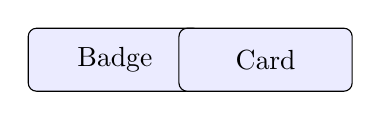
\begin{tikzpicture}
  \node[box] (a) {Badge};
  \node[box, right=-3mm of a] (b) {Card};
\end{tikzpicture}

\end{document}
